\section{Motivating Example}\label{motivExample}

Suppose that you are student in a School of Magic.
It is your first day in the School, so navigation in the building is a problem for you.
Fortunately, you have a map of the building (fig.~\ref{input}) and an additional knowledge about building construction:
\begin{itemize}
  \item there are towers in the school (nodes of the graph in your map);
  \item towers can be connected by directed galleries (edges in your map);
  \item galleries have a ``magic'' property: you can start from any floor, but following each gallery you either end one floor above (edge label is 'a'), either one floor below (edge label is 'b'). 
\end{itemize}

\begin{figure}[h]
    \begin{center}
        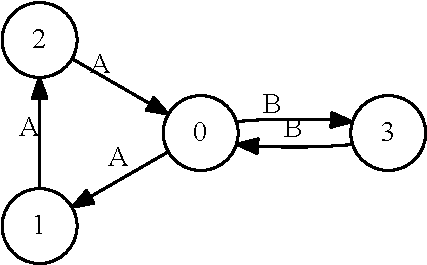
\includegraphics[width=6cm]{dot/input.pdf}
        \caption{The map of School (input graph $M$)}
        \label{input}        
    \end{center}
\end{figure}


You want to find a path from your current position to the same floor in another tower. 
Map with all such paths can help you.
But orienteering is not your forte, so it would be great if the structure of the paths were as simple as possible and all paths had additional checkpoints to control your rout.

It is evident that the simplest structure of required paths is $\{ab, aabb, aaabbb, \dots\}$.
In terms of our definitions, it is necessary to find all paths $p$ such that $\Omega(p) \in \{a^n b^n, n \geq 1\}$ in the graph $M=(\{0;1;2;3\},E,\{a;b\})$ (figure~\ref{input}).

Unfortunately, language $\mathcal{L} = \{a^n b^n; n \geq 1\}$ is not regular which restricts the set of tools you can use. 
Another problem is the infinite size of solution, but you want to get a finite map.  
Moreover, you want to know a structure of paths in terms of checkpoints.

We are not aware of any existing tools which can help to solve this problem and we create the such tool.
Let us to show how to get a map which helps to navigate in this strange School.

Fortunately, the language $\mathcal{L} = \{a^n b^n; n \geq 1\}$ is a context-free language and can be specified with context-free grammar. 
The fact that one language can be described with more than one grammar allows to add checkpoints: additional nonterminals can mark required parts of a sentence.
In our case, a desired checkpoint can be in the middle of the path.
As a result, required language can be specified by the grammar $G_1$ presented in figure~\ref{grammarG}, where $N = \{s; \text{\textit{Middle}}\}$, $\Sigma = \{a; b\}$, and $S$ is a start nonterminal.

\begin{figure}[h]
   \begin{center}
   \[
\begin{array}{rl}
   0:& S \rightarrow a \ S \ b \\
   1:& S \rightarrow Middle \\
   2:& Middle \rightarrow a \ b
\end{array}
\]

   \caption{Grammar $G_1$ for language $L=\{a^n b^n; n \geq 1\}$ with additional marker for a middle of a path}
   \label{grammarG}        
   \end{center}
\end{figure}

In the next section we present a map construction algorithm,  which solves such problems.
